\documentclass[12pt]{article}
\usepackage[utf8]{inputenc}
\usepackage{fullpage}
\usepackage{float}
\usepackage[a4paper, total={6in, 8in}]{geometry}
\usepackage{graphicx}
\usepackage{tikz}
\usepackage{amsmath}
\usepackage{array,multirow}
\usepackage{multicol}
\usetikzlibrary{shapes.geometric, arrows}

\tikzstyle{startstop}=[rectangle,rounded corners,minimum width=2cm,minimum height=1cm,text centered,draw=black,fill=red!30]
\tikzstyle{io}=[trapezium,trapezium left angle=70,trapezium right angle = 110,minimum width = 2cm, minimum height=1cm,text width=2cm,text centered, draw=black,fill=blue!30]
\tikzstyle{process}=[rectangle,minimum width=2cm,minimum height=1cm,text width=2cm,text centered,draw=black,fill=orange!30]
\tikzstyle{decision}=[diamond,minimum width=2cm,minimum height=1cm,text centered,text width=2cm,draw=black,fill=green!30]
\tikzstyle{arrow} = [thick,->,>=stealth]

\graphicspath{ {images/} }


\title{Flight Delay Prediction}
\author{S Saikrishnan}

\begin{document}

\maketitle

\begin{abstract}
The Federal Aviation Administration (FAA) considers a flight to be delayed when it takes off and/or lands 15 minutes later than its scheduled time. This project aims to predict if a flight is delayed and also find how long the flight was delayed using a two stage predictive model. This model is designed based on the data containing flights in USA and the weather data pertaining to 15 airports, both from 2016 and 2017. Based on this data, classifier predicts if the flight is delayed or not. If delayed, regressor predicts the delay. Out of various algorithms, random forest classifier (F1 score (0.78)) proved to be the best for classification and random forest regressor (R2 score (0.944)) proved to be the best for regression. 

\end{abstract}
\section{Introduction}
    Delays in flights can be caused due to various factors such as traffic volume, aircraft type, aircraft maintenance, airline operations and weather conditions. Studies show that weather conditions have contributed to 69\% of delays in flights. This project leverages the influence
    of the weather conditions in affecting the flight schedule, to predict if the flight was delayed and also find how long the flight was delayed.
    The project is divided into 3 modules,
\begin{center}
\begin{itemize}
        \item Data Preprocessing 
		\item Classification 
		\item Regression 
\end{itemize}
\end{center}


\section{Data Preprocessing}
Airports for which this data has been collected are represented by their corresponding Airport Codes as shown in Table \ref{Table:1}.
\begin{table}[H]
\begin{center}
\begin{tabular}{ |c|c|c| } 
\hline
 ATL & CLT & DEN \\ 
\hline
 DFW & EWR & IAH \\
\hline
 JFK & LAS & LAX \\
\hline
 MCO & MIA & ORD \\
\hline
 PHX & SEA & SFO \\ 
\hline
\end{tabular}
\caption{List of Airports}
\label{Table:1}
\end{center}
\end{table}
The flight data is collected for 24 months (2016-2017), from CSV files corresponding to each month and collectively made into a single dataset.  However, this dataset would contain many attributes out of which only those shown in Table \ref{Table:2} are filtered to make the final flight data.
\begin{table}[H]
\begin{center}
\begin{tabular}{ |c|c|c| } 
\hline
 FlightDate & Quarter & Year \\ 
 \hline
 Month & DayofMonth & DepTime \\
 \hline
 DepDel15 & CRSDepTime & DepDelayMinutes \\
 \hline
 OriginAirportID & DestAirportID & ArrTime \\
 \hline
 CRSArrTime & ArrDel15 & ArrDelayMinutes \\ 
 \hline
\end{tabular}
\caption{List of flight features}
\label{Table:2}
\end{center}
\end{table}
Weather data is given in the form of a JSON file from 2013-2017, month wise. This also made into a dataset containing hourly data from years (2016-2017) with features represented in Table \ref{Table:3}.
\begin{table}[H]
\begin{center}
\begin{tabular}{ |c|c|c| } 
 \hline
 WindSpeedKmph & WindDirDegree & WeatherCode \\ 
 \hline
 precipMM & Visiblity & Pressure \\
 \hline
 Cloudcover & DewPointF & WindGustKmph \\
 \hline
 tempF & WindChillF & Humidity \\
 \hline
 date & time & airport \\
 \hline
\end{tabular}
\caption{List of weather features}
\label{Table:3}
\end{center}
\end{table}
Since, the weather data is hourly, the departure time of the flights is approximated to the nearest hours. Flight data and weather data are merged based on Departure Airport, Departure Time and Date. This dataset is now considered as the final processed data that will be used for further modeling and predictions. It is ensured that there are no duplicates in this dataset to avoid redundancy, and the final data has 28 features and 18,34,170 data points. 80\% of these are used for training the model and the remaining 20\% is used as the test data to test the accuracy of the model.

\section{Classification}
The first step of the two-stage predictive model is classification, where the flights are  classified as delayed or not delayed.
\subsection{Metrics Used}
 TP (True Positive) denotes the delayed flights predicted correctly,\\
    TN (True Negative) denotes not delayed flights predicted correctly,\\
    FP (False Positive) denotes not delayed flights predicted incorrectly,\\
    FN (False Negative) denotes delayed flights predicted incorrectly.\\
$$Precision = \frac{TP}{TP+FP}$$
$$Recall = \frac{TP}{TP+FN}$$
$$F1\ Score =  \frac{2\times Precision\times Recall}{Precision+Recall}$$
$$Accuracy =\frac{TP+TN}{TP+TN+FP+FN}$$


\subsection{ Classifier Results}
\begin{table}[H]
\begin{center}
\begin{tabular}{ |c|c|c|c|c|c|c|c| }
\hline
 \multirow{2}{*}{\textbf{Algorithm}} & \multicolumn{2}{c|}{\textbf{Precision}} & \multicolumn{2}{c|}{\textbf{Recall}} & \multicolumn{2}{c|}{\textbf{F1-Score}} & \multirow{2}{*}{\textbf{Accuracy}} \\
 \cline{2-7}
        & 0 & 1 & 0 & 1 & 0 & 1 & \\
\hline
 Logistic Regression &  0.92 & 0.89 & 0.98 & 0.67 & 0.95 & 0.76 & 0.91\\
 \hline
 Decision Tree &  0.92 & 0.68 & 0.91 & 0.71 & 0.92 & 0.69 &  0.87\\
 \hline
 Extra Tree &  0.93 & 0.83 & 0.96 & 0.73 & 0.94 & 0.78 & 0.91\\
 \hline
 Random Forest & 0.92 & 0.89 & 0.98 & 0.70 & 0.95 & 0.78 & 0.92\\
\hline
\end{tabular}
\caption{Classifier scores}
\label{Table 4}
\end{center}
\end{table}
The observed scores for class 1 are much less compared to those of class 0. This is because the number of flights that are not delayed are more than the number of flights that are delayed. Distribution of the dataset is depicted in Fig \ref{fig:1}. \\
\begin{figure}[H]
    \centering
    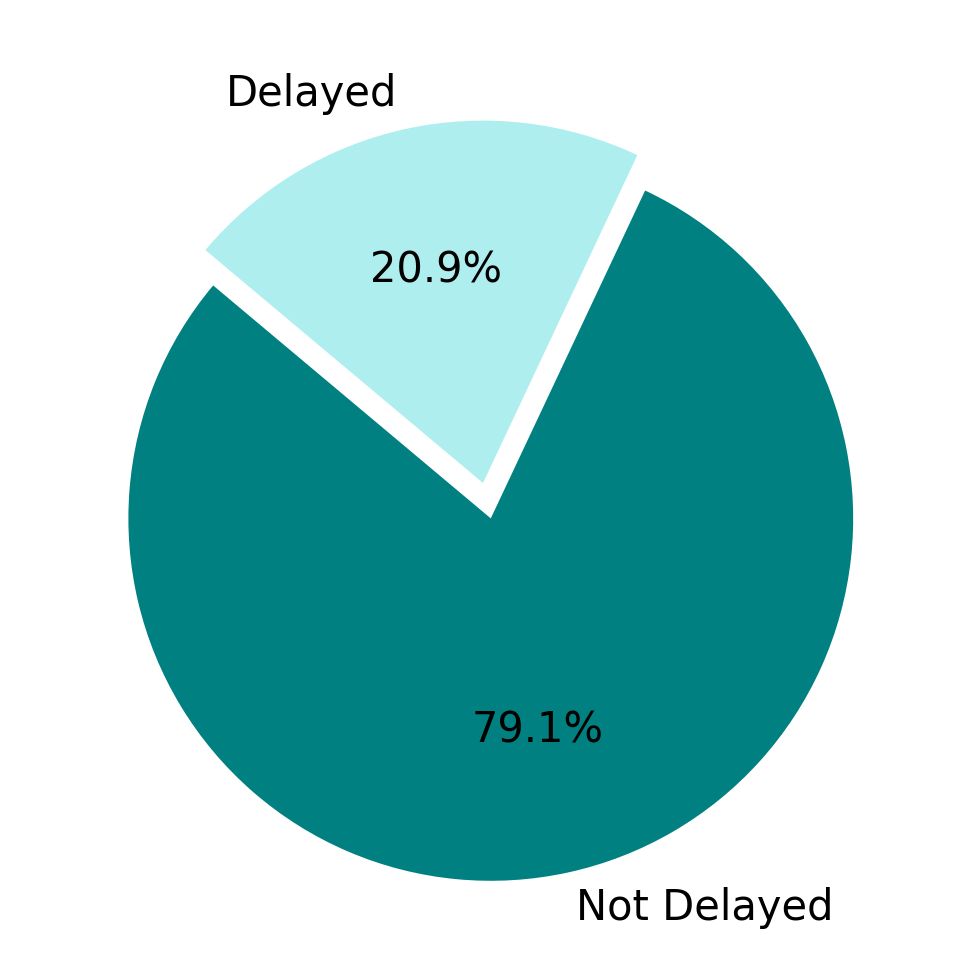
\includegraphics{Pie Chart of ArrDel15 Distribution.png}
    \caption{Pie Chart of ArrDel15 Distribution}
    \label{fig:1}
\end{figure}
This data imbalance calls for the need of sampling.
There are 2 types of sampling namely, Oversampling and
Undersampling. These are techniques used to adjust the class distribution of a dataset. Oversampling methods derive new examples from the existing datapoints in the minority class, whereas undersampling balances the dataset by eliminating datapoints from majority class. SMOTE was used for oversampling and Random Under Sampler was used for undersampling.\\
\begin{center}
         \textbf{Synthetic Minority Oversampling Technique} (SMOTE) works by selecting examples that are close in the feature space, drawing a line between the examples in the feature space and drawing a new sample at a point along that line.\\
\end{center}
\begin{table}[H]
\begin{center}
\caption{Scores after Oversampling}
\begin{tabular}{ |c|c|c|c|c|c|c|c| }
\hline
 \multirow{2}{*}{\textbf{Algorithm}} & \multicolumn{2}{c|}{\textbf{Precision}} & \multicolumn{2}{c|}{\textbf{Recall}} & \multicolumn{2}{c|}{\textbf{F1-Score}} & \multirow{2}{*}{\textbf{Accuracy}} \\
 \cline{2-7}
        & 0 & 1 & 0 & 1 & 0 & 1 & \\
\hline
Logistic Regression & 0.94 & 0.74 & 0.93 & 0.78 & 0.93 & 0.76 &  0.89\\
 \hline
 Decision Tree & 0.92 & 0.67 & 0.91 & 0.70 & 0.91 & 0.69 & 0.87\\
 \hline
 Extra Tree & 0.94 & 0.80 & 0.95 & 0.75 & 0.94 & 0.77 & 0.91\\
 \hline
 Random Forest & 0.93 & 0.85 & 0.97 & 0.72 & 0.95 & 0.78 & 0.92\\
\hline
\end{tabular}
\label{Table 5}
\end{center}
\end{table}
     In \textbf{Random Under-Sampling}, the majority class instances are discarded at random until a more balanced distribution is reached. It is repeated until the desired class distribution is achieved in the training dataset, such as an equal split across the classes.
\begin{table}[H]
\begin{center}
\caption{Scores after undersampling}
\begin{tabular}{ |c|c|c|c|c|c|c|c| }
\hline
 \multirow{2}{*}{\textbf{Algorithm}} & \multicolumn{2}{c|}{\textbf{Precision}} & \multicolumn{2}{c|}{\textbf{Recall}} & \multicolumn{2}{c|}{\textbf{F1-Score}} & \multirow{2}{*}{\textbf{Accuracy}} \\
 \cline{2-7}
        & 0 & 1 & 0 & 1 & 0 & 1 & \\
 \hline
 Logistic Regression & 0.94 & 0.74 & 0.93 & 0.78 & 0.93 & 0.76 & 0.90\\
 \hline
 Decision Tree & 0.94 & 0.51 & 0.79 & 0.80 & 0.86 & 0.62 &  0.79\\
 \hline
 Extra Tree & 0.95 & 0.67 & 0.89 & 0.82 & 0.92 & 0.74 & 0.88\\
 \hline
 Random Forest & 0.95 & 0.71 & 0.91 & 0.81 & 0.93 & 0.76 & 0.89\\
\hline
\end{tabular}
\label{Table 6}
\end{center}
\end{table}
\subsection{Observations}
Table \ref{Table 5} shows the results for the different models used for the classifier after oversampling and it is observed that there is an increase in scores for class labelled 1, in Logistic Regression.\\
Table \ref{Table 6} shows results after undersampling and it is observed that the scores for class labelled 1 have improved after sampling. It is also inferred that the oversampled Random Forest model is the best classifier as it has the highest F1 score corresponding to class 1.

\section{Regression}
The second of the two-stage predictive model is the regressor which predicts the delay on arrival (in minutes), for those flights which are classified under the ``Delayed`` class by the Classifier. Since only the delayed flights are considered, the remaining flights are removed to make a subset of the original dataset,  which is again split in the ratio 80:20 for train and test sets respectively of the regressor model.\\
\subsection{Metrics Used}
$y_{1}$, $y_{2}$, $y_{3}$, ..., $y_{n}$ are values predicted by the regressor.\\
$x_{1}$, $x_{2}$, $x_{3}$, ..., $x_{n}$ are actual values.\\
 n is the number of observations.\\ 
$$Mean\ (\overline{x}) =(\frac{1}{n})\sum_{i=1}^{n}(x_{i})$$
$$Root\ Mean\ Square\ Error\ (RMSE) =\sqrt{(\frac{1}{n})\sum_{i=1}^{n}(y_{i} - x_{i})^{2}}$$
$$Mean\ absolute\ Error\ (MAE)=(\frac{1}{n})\sum_{i=1}^{n}\left | y_{i} - x_{i} \right |$$
$$R\ Squared\ (R2)= 1 - \frac{\sum_{i=1}^{n}(y_{i} - x_{i})^{2}}{\sum_{i=1}^{n}(y_{i} - \overline{x})^{2}}$$ 
 
\subsection{Regressor Results}
\begin{table}[H]
    \centering
    \begin{tabular}{|c|c|c|c|}
    \hline
    \textbf{Regressor} & \textbf{RMSE} & \textbf{MAE} & \textbf{R2 Score} \\
    \hline
    Linear Regression & 17.50 & 12.19 & 0.938 \\
    \hline
    ExtraTree & 16.83 & 11.87 & 0.943 \\
    \hline
    Random Forest & 16.64 & 11.72 & 0.944 \\
    \hline
    Gradient Boost & 16.80 & 11.66 & 0.943 \\
    \hline
    \end{tabular}
    \caption{Regressor Scores}
    \label{tab:Table 7}
\end{table}
R-squared (R2) is a statistical measure that represents the proportion of the variance for a dependent variable in a regression model.
Table \ref{tab:Table 7} gives the performance of the different models used for the Regressor and it is observed that the Random Forest has the best performance with R2 value 0.944 and RMSE 16.64.
\subsection{Regression Analysis}
The dataset was split into ranges of \textbf{ArrDelayMinutes} and performance of the model is tested in the ranges given in Table \ref{tab:Table 8}.
\begin{table}[H]
    \centering
    \begin{tabular}{|c|c|c|}
    \hline
        \textbf{Ranges} & \textbf{RMSE} & \textbf{MAE} \\
    \hline
        0-100 & 13.69 & 10.25 \\
    \hline
        100-200 & 18.35 & 14.43\\
    \hline
        200-500 & 27.06 & 19.34\\
    \hline
        500-1000 & 20.98 & 16.01\\
    \hline
        1000-2000 & 62.61 & 25.69\\
    \hline
    \end{tabular}
    \caption{Regression Testing}
    \label{tab:Table 8}
\end{table}
From Table \ref{tab:Table 8}, it is clear that the errors increase with increase in arrival delay minutes. This is because, the number of datapoints in the range (0-100) and (100-200) is much more compared to the higher ranges, shown in frequency distribution plot (Figure \ref{fig:2}). But the relative errors decrease with increasing ranges. 25.69 MAE for range(1000 - 2000) is better than 10.25 MAE for (0-100).
\begin{figure}[H]
    \centering
    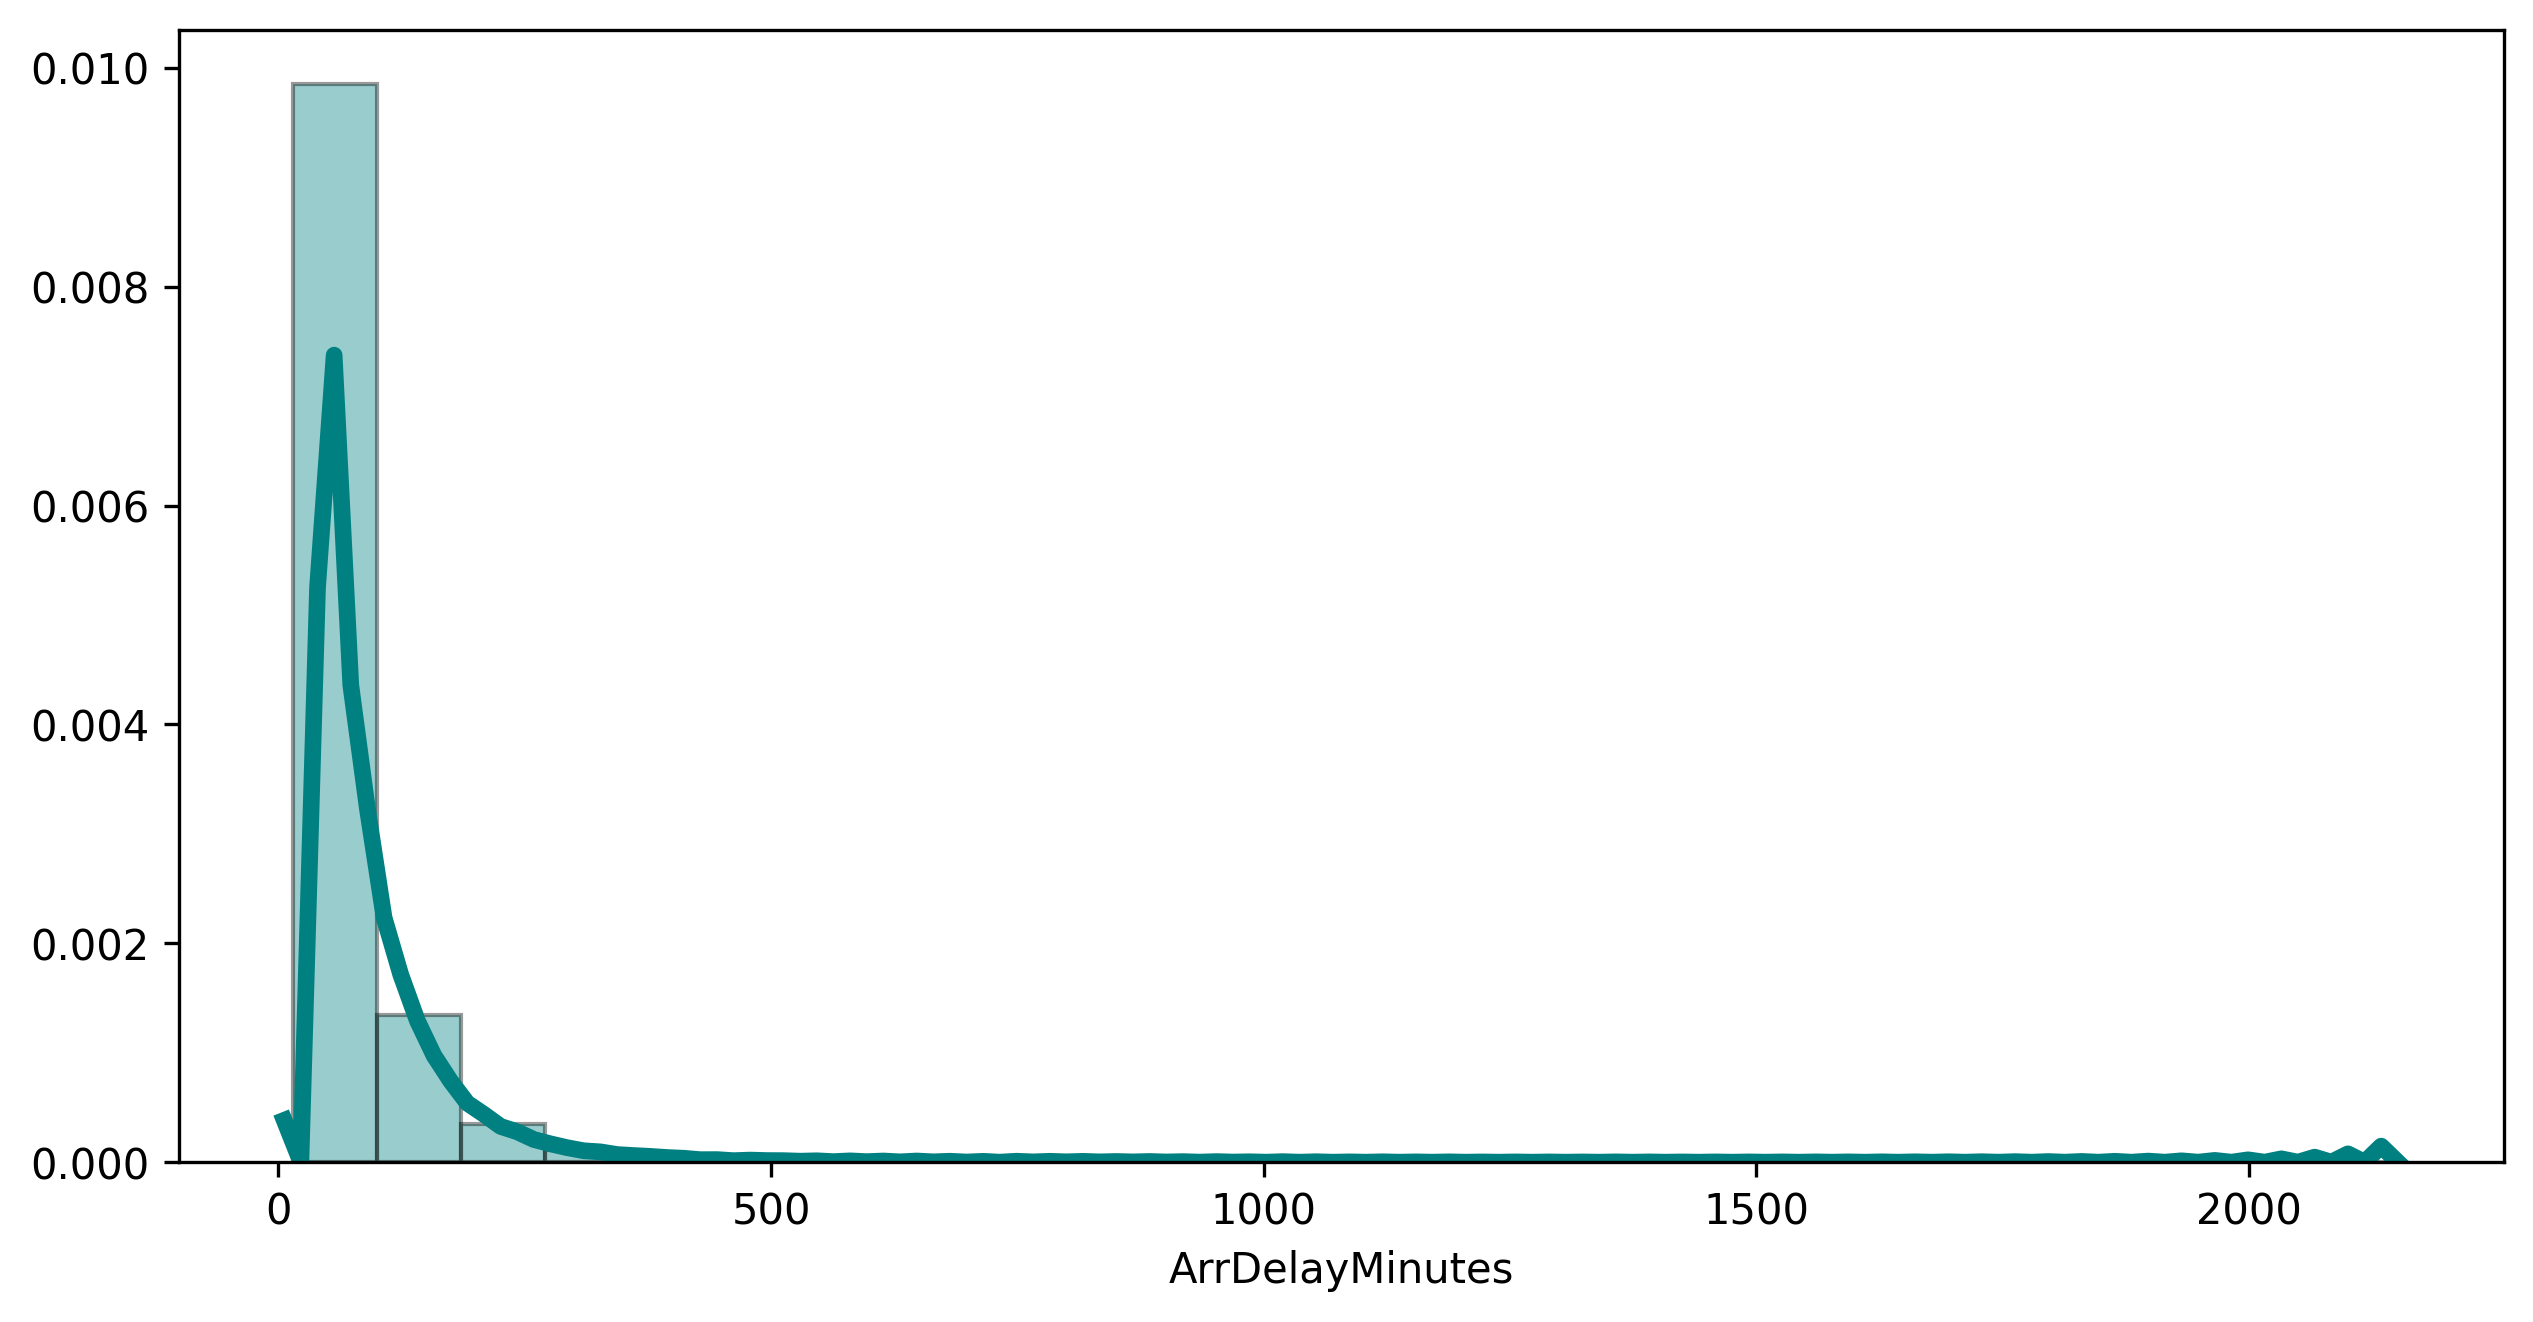
\includegraphics[scale=.5]{Frequency Distribution of ArrDelayMinutes.png}
    \caption{Frequency Distribution of `ArrDelayMinutes`}
    \label{fig:2}
\end{figure}
\section{Pipeline}
The best classifier is chosen and fed to the best regressor, (here both being Random Forest), forms the basis for the functioning of the pipeline(shown in the flowchart given below) and hence completes the two-staged model.\\

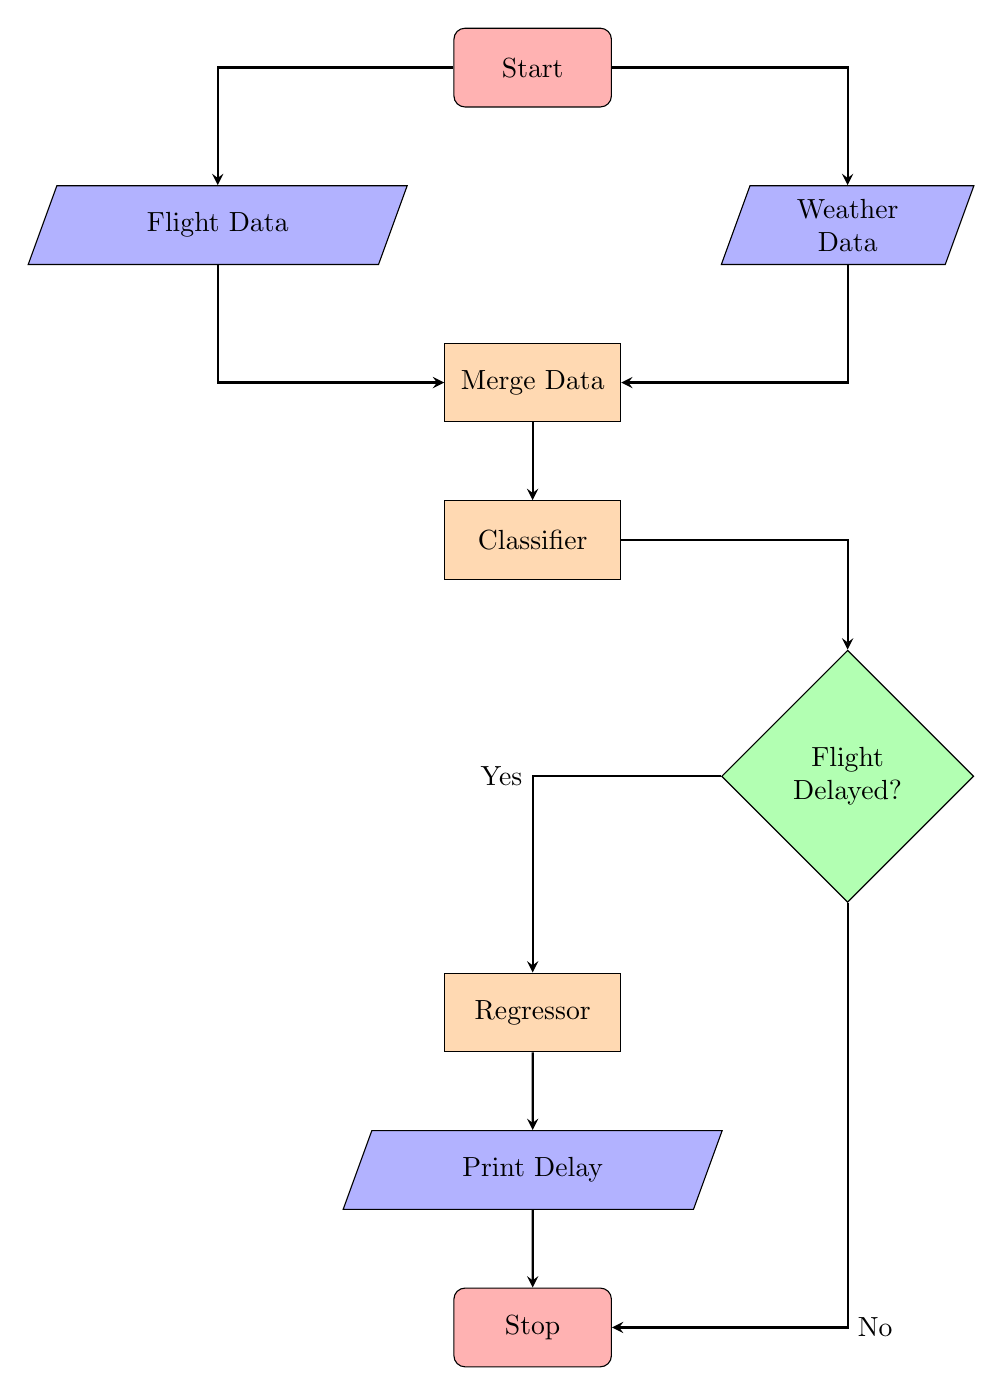
\begin{tikzpicture}[node distance = 2cm]

\node (start) [startstop]{Start};
\node (in1) [io,below of =start,xshift=-4cm]{Flight Data};
\node (in2) [io,below of =start,xshift=4cm]{Weather Data};
\node (pro1) [process,below of =in1,xshift=4cm]{Merge Data};
\node (pro2) [process,below of =pro1]{Classifier};
\node (dec1) [decision,below of =pro2,yshift=-1cm,xshift=4cm]{Flight Delayed?};
\node (pro3) [process,below of =dec1,yshift=-1cm,xshift=-4cm]{Regressor};
\node (out1) [io,below of =pro3]{Print Delay};
\node (stop) [startstop,below of =out1]{Stop};

\draw[arrow] (start) -| (in1);
\draw[arrow] (start) -| (in2);
\draw[arrow] (in1) |- (pro1);
\draw[arrow] (in2) |- (pro1);
\draw[arrow] (pro1) -- (pro2);
\draw[arrow] (pro2) -| (dec1);
\draw[arrow] (dec1) -| node[anchor=east]{Yes} (pro3);
\draw[arrow] (pro3) -- (out1);
\draw[arrow] (out1) -- (stop);
\draw[arrow] (dec1) |- node[anchor=west]{No} (stop);
\end{tikzpicture}
\begin{table}[H]
    \centering
    \caption{Scores after Pipeline}
    \begin{tabular}{|c|c|c|c|}
    \hline
         \textbf{Regressor} & \textbf{RMSE} & \textbf{MAE} & \textbf{R2 Score} \\
    \hline
        Random Forest & 13.24 & 8.79 & 0.97 \\
    \hline
    \end{tabular}
    \label{tab:Table 9}
\end{table}
\section{Conclusion}
  The flight data and the weather data were processed and merged based on airport, date and departure time. The classifier was trained using this data and it was found that classifier performed poorly for the minority class in the dataset due to data imbalance. Sampling the data points using SMOTE and random undersampling improved the scores for the minority class. The best classifier, Random Forest Classifier having F1 score (0.78) and accuracy (0.92), was chosen and pipelined with the best regressor, Random Forest Regressor having R2 score (0.944) and RMSE (16.64) to form the pipelined architecture. The performance of the two staged pipelined model was analyzed. The pipeline model had higher scores, RMSE (13.24) and R2 score (0.97).
\end{document}